\documentclass[tikz,border=2pt]{standalone}
\usepackage{amsmath,amssymb}
\usepackage{tikz}
\usepackage{pgfplots}
\pgfplotsset{compat=1.18}

\begin{document}
% The critical ratio beta = b/(b+h) is the probability level at which the demand CDF is cut:
% meals with b = 3.3, h = 2.2 give beta = 0.6; uniform demand on [80,120] gives y* = 104.
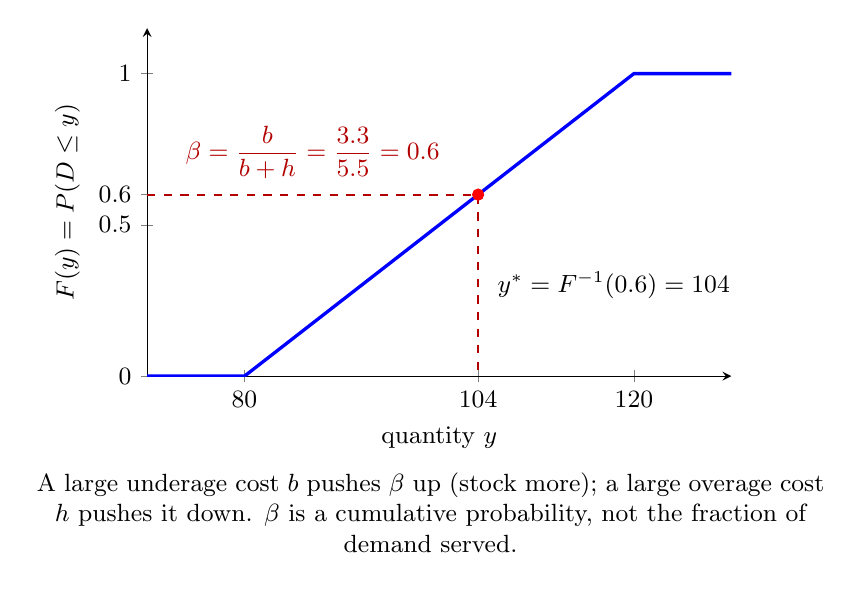
\begin{tikzpicture}
	\begin{axis}[width=9cm, height=6cm, xlabel={quantity $y$}, ylabel={$F(y)=P(D\le y)$}, xmin=70, xmax=130, ymin=0, ymax=1.15, axis lines=left, tick label style={font=\small}, label style={font=\small}, xtick={80,104,120}, ytick={0,0.5,0.6,1}]
		\addplot[blue, very thick] coordinates {(70,0) (80,0) (120,1) (130,1)};
		\draw[red!70!black, dashed, thick] (axis cs:70,0.6) -- (axis cs:104,0.6) -- (axis cs:104,0);
		\addplot[only marks, mark=*, mark size=2pt, red] coordinates {(104,0.6)};
		\node[anchor=south, font=\small, red!70!black] at (axis cs:87,0.62) {$\beta=\dfrac{b}{b+h}=\dfrac{3.3}{5.5}=0.6$};
		\node[anchor=west, font=\small] at (axis cs:105,0.3) {$y^*=F^{-1}(0.6)=104$};
	\end{axis}
	\node[anchor=north, align=flush center, text width=10cm, font=\small] at (3.6,-1.1) {A large underage cost $b$ pushes $\beta$ up (stock more); a large overage cost $h$ pushes it down. $\beta$ is a cumulative probability, not the fraction of demand served.};
\end{tikzpicture}
\end{document}
